\documentclass{ctexart}
\usepackage{EC}
\begin{document}
\section{硅及其化合物}
\subsection{硅单质}
\subsubsection{硅单质的制备}
\paragraph{硅单质的发现}
从硅酸盐矿物中得到硅单质的历史已有两百余年.1808年,Berzelius就尝试用\ce{Fe}和\ce{C}的混合物还原石英\ce{SiO2}以得到\ce{Si}单质,但可惜的是显然他得到的是硅铁.1809年,Davy也从事\ce{Si}单质的制备,但也没有成功.\\
\indent 1811年,Gay Lussac和Thénard用金属钾还原\ce{SiCl4},得到了一种无定形的棕色粉末:
\begin{center}
    \ce{4K + SiCl4 -> 4KCl + Si}
\end{center}
可惜的是,他们并没有认出这种棕色粉末就是硅单质.直到1823年,Berzelius重新用\ce{K}单质还原\ce{K2SiF6}而制得了\ce{Si}单质:
\begin{center}
    \ce{4K + K2SiF6 -> 6KF + Si}
\end{center}
他还对产物进行了细致的清洗,并研究了硅单质的若干性质.因此,一般将\ce{Si}单质的发现人归为Berzelius.
\paragraph{硅单质的工业制备方法I}
\indent 继最早的研究之后,又有发现了许多制备\ce{Si}单质的方法,主要是用碱金属或碱土金属作为还原剂还原含\ce{Si}化合物,或采取放电还原的方式.现在,在工业上制备\ce{Si}单质的方法为将焦炭与过量的\ce{SiO2}共热:
\begin{center}
    \ce{SiO2 + 2C ->T[$\Delta$] Si + 2CO}
\end{center}
显然地,\ce{SiO2}过量可以防止难以分离的\ce{SiC}的生成.这样得到的硅单质纯度大约为$97\sim98\%$.将其熔融后重结晶,再经过酸洗后即得到纯度为$99.7\sim99.8\%$的纯硅.如果需要制得高纯度的半导体硅,首先可以用\ce{HCl}与\ce{Si}单质反应得到\ce{SiHCl3}:
\begin{center}
    \ce{Si + 3HCl ->T[$280\sim320\tc$][\ce{CuCl}] SiHCl3 + H2}
\end{center}
随后将得到的混合物(其中的主要杂质是其它元素的氯化物,例如\ce{AlCl3}等)进行精馏而得到较纯的\ce{SiHCl3},然后在高温下用\ce{H2}还原并采取气相沉积法(CVD)收集\ce{Si}即可得到多晶\ce{Si}单质:
\begin{center}
    \ce{SiHCl3 + H2 ->T[$1100\tc$] Si + 3HCl}
\end{center}
这样制得的硅单质纯度在$\underbrace{99.99999}_{\text{7个9}}\%$到$\underbrace{99.9999999}_{\text{9个9}}\%$左右.通常,我们用$xN$表示硅单质杂质含量少于$10^{-x}$,因此这样制得的多晶硅纯度为$7N$到$9N$.
\paragraph{硅单质的工业制备方法II}
如果想要制备纯度为$11N$及以上的单晶硅,还需要区域熔炼法或提拉法继续提纯.\\
\indent 提拉法又称柴可拉斯基法(Czochralski Process),其过程如下所示.
\chemfig{Czochralski_Process}{0.4}{提拉法的步骤示意图}
提拉法的步骤为:
\begin{enumerate}[label=$\mathit{Step\ \arabic*.}$,topsep=0pt,parsep=0pt,itemsep=0pt,partopsep=0pt,leftmargin=*]
    \item 将高纯度的多晶硅在坩埚(通常是石英坩埚)中熔融.有时需要按照用途掺杂.
    \item 将晶种连接在一根精确定向的棒的末端.
    \item 使棒的末端浸入熔融的硅单质中.
    \item 缓慢向上提拉棒,同时匀速旋转棒.控制旋转速率,提拉速率和温度,即可在相界面上不断结晶出高纯度的,一定半径的\ce{Si}单质棒.
    \item 将棒与\ce{Si}单质截断,即可得到单晶\ce{Si}.通常,这样的\ce{Si}单质可以被直接切割为晶圆(即圆形的单晶\ce{Si}薄片),然后用于芯片等的生产.
\end{enumerate}

\indent 区域熔炼法则是根据相平衡的原理进行提纯的.我们以提纯\ce{Si}为例,其中的杂质的存在将导致凝固点发生变化.
\begin{figure}[H]
    \centering\documentclass{standalone}
\usepackage{PhysicalChemistryNote}
\begin{document}
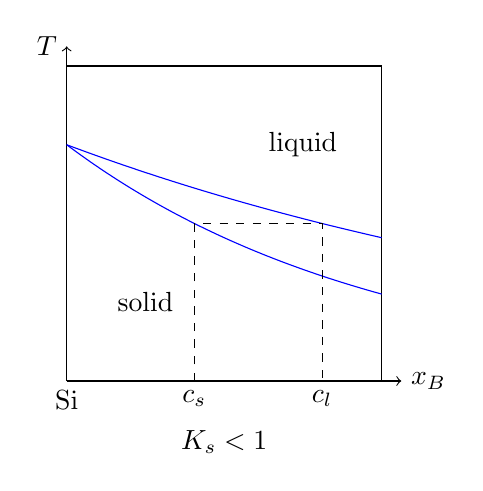
\begin{tikzpicture}
    \draw[->] (0,0) -- (4.25,0) node[right] {$x_B$};
    \draw[->] (0,0) -- (0,4.25) node[left]{$T$};
    \draw[-] (4,0) -- (4,4);
    \draw[-] (0,4) -- (4,4);
    \node[below] at (0,0) {Si};
    \draw[domain=0:4,blue] plot[smooth](\x,{3*e^(-\x/4)});
    \draw[domain=0:4,blue] plot[smooth](\x,{3*e^(-\x/8)});
    \draw[dashed] (1.6218,0)--(1.6218,2)--(3.2437,2)--(3.2437,0);
    \node[below] at (1.6218,0) {$c_{\text s}$};
    \node[below] at (3.2437,0) {$c_{\text l}$};
    \node[below] at (2,-0.5) {$K_s<1$};
    \node at (1,1) {solid};
    \node at (3,3) {liquid};
\end{tikzpicture}
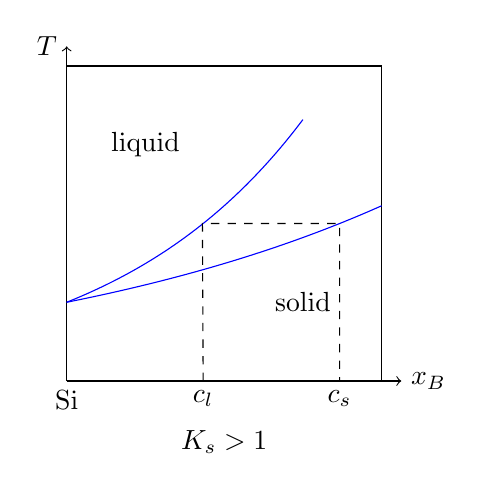
\begin{tikzpicture}
    \draw[->] (0,0) -- (4.25,0) node[right] {$x_B$};
    \draw[->] (0,0) -- (0,4.25) node[left]{$T$};
    \draw[-] (4,0) -- (4,4);
    \draw[-] (0,4) -- (4,4);
    \node[below] at (0,0) {Si};
    \draw[domain=0:3,blue] plot[smooth](\x,{e^(\x/2.5)});
    \draw[domain=0:4,blue] plot[smooth](\x,{e^(\x/5)});
    \draw[dashed] (1.7329,0)--(1.7239,2)--(3.4657,2)--(3.4657,0);
    \node[below] at (1.7329,0) {$c_{\text l}$};
    \node[below] at (3.4657,0) {$c_{\text s}$};
    \node[below] at (2,-0.5) {$K_s>1$};
    \node at (3,1) {solid};
    \node at (1,3) {liquid};
\end{tikzpicture}
\end{document}
    \caption{熔融液体凝固时固相中的杂质含量变化}
\end{figure}
图中纵坐标为温度,横坐标为杂质$B$的含量$x_B$,在固相线和液相线之间为两相共存区.在一定温度下,令杂质在固相和液相中的浓度为$c_{\text s}$和$c_{\text l}$.设\tbf{分凝系数}$K_s$满足
\[K_s=\dfrac{c_{\text s}}{c_{\text l}}\]
\indent 先讨论$K_s<1$的情形.假设熔炼区域从左向右移动,那么在熔融区的左侧正在发生重新凝固.凝固时,固相中杂质的浓度小于液相,因此杂质更多地被分配在液相中,于是随着熔炼区域的右移而右移.这样多次重复后,杂质就被扫到最右侧,而左侧就是纯度较高的物质.\\
\indent 对于$K_s>1$的情形,杂质更多地被分配在重新凝固的左侧,因此右侧是纯度较高的物质.\\
\indent 在\ce{Si}中,所有杂质的$K_s<1$,所以经过区域熔炼后杂质集中在尾部.对于\ce{Ge}而言,\ce{B}和\ce{Si}的$K_s>1$,其余杂质的$K_s<1$,因此纯的\ce{Ge}集中在中部,应弃去头尾.\\
\indent 区域熔炼的效率一方面取决于$K_s$的大小,一方面取决于提纯前物质的纯度.$K_s$越远离$1$,提纯前的物质越纯,区域熔炼的效率越高.于是进行区域熔炼法之前一般要用其他方法,例如化学法进行提纯.\\
\indent 区域熔炼法也可以用于有机物的提纯和高分子化合物的分类,并且能达到很好的效果,因为区域熔炼法可以重复多次.
\subsubsection{硅单质的结构}
一般的单晶硅与金刚石的结构相似,以立方金刚石结构为主.
\chemfig{Si}{0.1}{单晶硅的晶体结构}
由于单晶硅的表面性质与表面的方向密切相关,因此这里简单地介绍一些有关晶面的知识.\\
\indent 晶面是晶体中由周期性排列的原子所形成的几何平面,它反映了晶体内部结构的对称性与规律性,同时对晶体的物理和化学性质有重要影响.例如解理面往往就是特定的晶面.\\
\indent 为了精确描述晶面取向,人们引入了密勒指数(Miller indices).密勒指数用一组三个整数 
$(hkl)$表示某一晶面,其确定方法为:
\begin{enumerate}[label=$\mathit{Step\ \arabic*.}$,topsep=0pt,parsep=0pt,itemsep=0pt,partopsep=0pt,leftmargin=*]
    \item 确定
\end{enumerate}
\end{document}